\documentclass[12pt]{article}
\usepackage[utf8]{inputenc}
\usepackage[T1]{fontenc}
\usepackage[brazil]{babel}
\usepackage{geometry}
\usepackage{graphicx}
\usepackage{booktabs}
\usepackage{hyperref}
\usepackage{url}

\geometry{a4paper, margin=2.5cm}

\title{Bitcoin: A História em Dados}
\author{Bruce Trevisan \\ Nicolas Palombo Lucas \\ Otávio Ribeiro Mello \\ Rafael Gomes Carneiro}
\date{ME115B - Linguagem R \\ Tatiana Andrea Benaglia Carvalho \\ Campinas, 2025}

\begin{document}

% Página de capa separada
\begin{titlepage}
    \centering
    {\LARGE\bfseries Bitcoin: \\ A História em Dados \par}
    \vspace{2cm}
    {\large Autores: \par}
    {\large Bruce Trevisan \par}
    {\large Nicolas Palombo Lucas \par}
    {\large Otávio Ribeiro Mello \par}
    {\large Rafael Gomes Carneiro \par}
    \vspace{3cm}

    \begin{minipage}{0.3\textwidth}
        \centering
        
\includegraphics[width=0.8\linewidth]{Imagens/unicamp-logo.png}
    \end{minipage}
    \hspace{5mm}
    \begin{minipage}{0.3\textwidth}
        \centering
        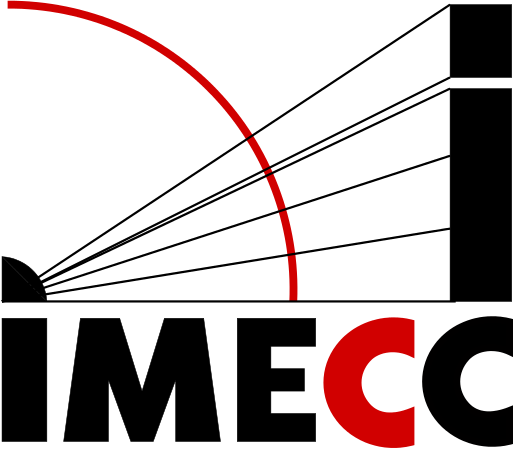
\includegraphics[width=0.8\linewidth]{Imagens/imecc-logo.png}
    \end{minipage}

    \vspace{2cm}
    {\large ME115B - Linguagem R \par}
    {\large Tatiana Andrea Benaglia Carvalho \par}
    \vfill
    {\large Campinas, 2025 \par}
\end{titlepage}

% Início do conteúdo em nova página
\newpage

\section*{Resumo}

\section*{Introdução}

\subsubsection*{O que são criptomoedas?}
Por definição, criptomoedas são qualquer tipo de moeda digital ou virtual que utiliza criptografia para garantir a realização de transações. Elas não têm autoridade central de emissão e sem regulação. Em contrapartida, elas utilizam um sistema de criptografia chamado de blockchain, além de outros sistemas de criptografia descentralizados para registrar transações e emitir novas unidades. 
\textbf{Blockchain é um banco de dados distribuído que consegue fazer um} compartilhamento de informações dentro de uma rede. Essas informações podem ser variadas, agrupadas em bloco a partir de criptografia, de uma forma que consiga trazer consigo o histórico completo e imutável das transações anteriores. Garantindo uma rede de operações concisas, seguras e confiáveis para qualquer um que desejar entrar nessa rede.

As criptomoedas atuam com diversas funções e objetivos além de um simples meio de transação monetária para uso diário. Elas podem ser reserva de valores; atuação como \textbf{ações de investimento}, por conta de sua alta volatilidade de seu valor; descontos em taxas; garantia de algum serviço; entre muitas outras funções.

Um dos maiores exemplos de criptomoedas são o Bitcoin e o Ether. O Ether valendo cerca de 2,6 mil dólares americanos, \textbf{\#MUDAR DEPOIS\#} além do Bitcoin, tendo mais de 100 mil dólares americanos \textbf{\#MUDAR DEPOIS\#} e sendo a criptomoeda mais famosa do mundo.

\subsubsection*{O que é bitcoin?}
Lançado em 2008, com o pseudônimo de Satoshi Nakamoto, uma nova ideia foi criada e posta ao mundo, com a criação do Bitcoin. O Bitcoin é atualmente a criptomoeda mais famosa do mundo, além de ser a mais valorizada atualmente, superando a marca de US\$100.000,00 
\textbf{\#MUDAR DEPOIS\#}

Devido ao fato do Bitcoin ser uma criptomoeda, logo, ela não tem uma emissão regularizada e centralizada, a emissão de novas moedas no mercado é de uma outra forma. É usado o termo "mineração". Esse processo consiste na resolução de quebra-cabeças matemáticos complexos feitos por hardware e software especializados para a mineração de Bitcoin. A mineração não é exclusiva de um grupo de pessoas, empresas ou bancos. Contanto que tenha energia e um hardware de mineração, é possível obter um bloco de Bitcoin.

Os blocos de bitcoin são os produtos e agrupamentos de transações individuais dos últimos dez minutos de cada mineração. Cada bloco é único e fechado, cada um criando seu próprio número \textit{Hash}, que é onde estão codificadas as transações. Cada novo bloco precisa ter em seu conteúdo as informações do bloco anterior, o que garante uma veracidade de que não será manipulado ou alterado. Cada bloco gerado é equivalente a uma quantidade específica de Bitcoin, cada bloco tem atualmente 3.125 BTC (Bitcoin).

Com tal unicidade, garante uma individualidade perante cada unidade de moeda não seja possuída por mais de um portador. O que torna a concorrência de cada máquina para garantir seu bloco próprio maior ainda, incentivando cada vez mais a melhora dos computadores para fazer a mineração. Além disso, para a autenticação no sistema de Prova de Trabalho (PoW) do Bitcoin, os computadores de mineração precisam comprovar a energia gasta para a mineração de cada bloco. O que reforça a segurança e autenticidade de cada máquina e bloco minerado.

\subsubsection*{O que é o Evento Halving?}
O evento Halving é um acontecimento periódico em que o número de Bitcoins em cada bloco minerado é reduzido pela metade, ocorre especificamente a cada 210 mil blocos minerados. Apesar de sua data não ser totalmente certa, é possível estimar com grande precisão, normalmente ocorrendo a cada 4 anos.

Seu objetivo é tentar controlar o valor da moeda com a inflação. O Halving não possui relações diretas no desejo de aumentar diretamente o valor de mercado da moeda, suas intenções valem tentativa de controle sobre o valor da moeda com a inflação. Adicionando o fato de que seu(s) criador(es) já deixaram bem explícito que haverá uma quantidade limitada de unidades de bitcoin, o que já está fixo na quantidade de 21 milhões.

Os efeitos do halving influenciam em seu valor indiretamente, já que pela lei da oferta e demanda, com a queda da oferta sobre o bitcoin e que normalmente há um aumento na demanda, seu preço aumenta.

Ele já ocorreu 4 vezes. Em 2012, 2016, 2020 e 2024.

% Tabela da Linha do Bitcoin Halving (Atualizar quando Bruce terminar a imagem)
\textbf{\#ATUALIZAR DEPOIS\#}

\begin{figure}[h]
    \centering
    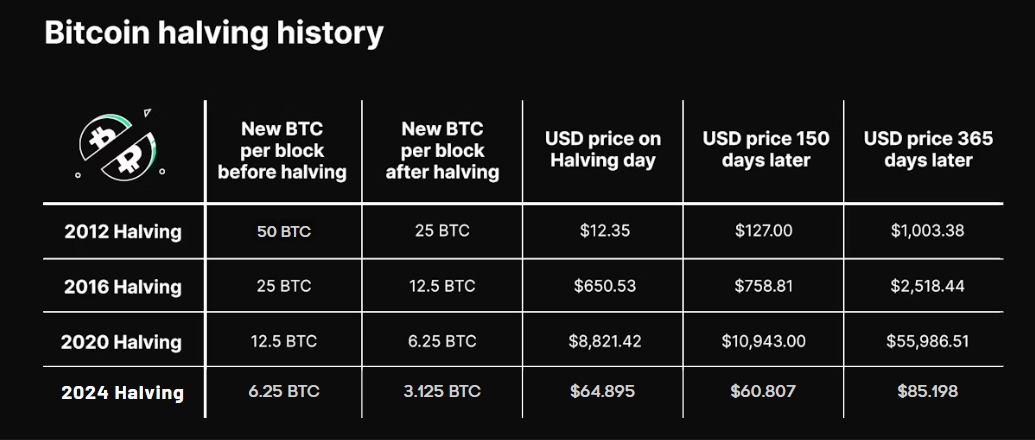
\includegraphics[width=0.8\textwidth]{Imagens/Bitcoin-halving-history.jpg}
    \caption{Tabela Cronológica do Evento Halving}
    \label{fig:Tabela Cronologica do Evento Halving}
\end{figure}

\newpage

\section*{Material e Métodos:}
% Material e Métodos: Descrição dos dados utilizados (origem, estrutura, principais variáveis). Explicação das técnicas aplicadas e do uso da linguagem R. Pacotes e funções principais empregados na análise.
% Não vai dar muito tempo de eu começar. Eu vou primeiro só organizar de como eu farei depois

\subsection*{Material utilizado:}

\subsection*{Metodologia:}

\subsection*{Códigos utilizados:}

\subsection*{Analise e Observações Interessantes}



\newpage % Limparr visualmente no pdf.


\section*{Resultados:}

\section*{Considerações Finais:}

\section*{Referências:}
\begin{itemize}
    \item \url{https://www.sciencedirect.com/science/article/pii/S1877343517300015}
    \item \url{https://blog.nubank.com.br/o-que-e-bitcoin/}
    \item \url{https://www.bbc.com/portuguese/internacional-57238550}
    \item \url{https://www.kaspersky.com.br/resource-center/definitions/what-is-cryptocurrency}
    \item \url{https://www.itau.com.br/investimentos/criptoativos}
    \item \url{https://content.btepactual.com/blog/conceitos-basicos/ativos-financeiros-o-que-sao-principais-ativos-e-como-escolher}
    \item \url{https://content.btepactual.com/blog/criptomocdas/entenda-o-que-sao-criptomocdas-e-qual-a-sua-utilidade}
    \item \url{https://www.infomoney.com.br/guias/halving-do-bitcoin/}
    \item \url{https://www.btipanda.com/academy/en/lessons/what-is-a-bitcoin-halving-and-what-happens-on-the-network/}
    \item \url{https://www.investopedia.com/terms/b/block-bitcoin-block.asp}
    \item \url{https://www.gemini.com/pt-BR/cryptopedia/what-is-block-in-blockchain-bitcoin-block-size}
    \item \url{https://www.investopedia.com/terms/m/mt-gox.asp}
    \item \url{https://exame.com/tecnologia/roubo-de-us-388-milhoes-em-bitcoins-leva-mt-gox-a-fechar/}
    \item \url{https://br.cointelegraph.com/news/the-mess-that-was-mt-gox-four-years-on}
\end{itemize}

\end{document}